\section{Makanya}

\subsection{Hintergrund} % Makanya
Der Hintergrund des Makanya.com Projektes ist eine Partnerschaft zwischen der Kirchengemeinde Kühlungsborn und Tansania,
sowie der Partnerschaft zwischen der Kirchengemeinde und dem Schulzentrum Kühlungsborns.
Der Pastor Kühlungsborns, Matthias Borchert,
suchte den Kontakt zum \jf Team über das Schulzentrum.
Nach einer kurzen Bekanntmachung durch Frau Schmidt war die Zusammenarbeit besiegelt.\\
Die Sachlage vor unserem Eintritt in das Projekt war eine Domain (\link{makanya.com}) von strato.de % TODO Quelle + Preise
% Server: strato.de
und ein WordPress Blog \link{kulungsi.de}. % FIXME Check TLD
Meine Aufgabe war es nun den Blog auf den technisch neusten Stand zu bringen und eine Website auf Makanya.com einzurichten.
Diese Website sollte dann als Anlaufpunkt für alle Projektteilnehmer, Interessenten und Schüler sein.
% Sprache: Deutsch, Englisch, Zusammenarbeit (Dolmetschering: Frau Wieck)
Aus dieser Spezifizierung ergeben sich die Anforderungen an die Programmierung:\\
Der Inhalt der Website muss auf Deutsch und Englisch sein, beide Versionen weitestgehend identisch.
Weiterhin soll die Webseite einfach bedienbar sein,
damit auch technisch unbegabte Schüler und Verwaltungsmitglieder sich durch die Webseite navigieren können sollen.
Damit die Seite auch in Tansania erreichbar ist müssen die Datenformate optimiert werden.\\
% Programmierung: PHP, HTML, MySQL
% Mehr Programmierung...?
% Beiprogramm: Schulzentrum -> Spendenlauf, Besuch der Tansanianer, Meetings, Auswertung
Somit stellt diese Arbeit ein Teil einer größeren Projektes dar.
Dieses Projekt beinhaltet die Partnerschaft von der Kirchengemeinde mit dem Schulzentrum und Makanya in Tansania.
Andere Aspekte beinhalten den Schüleraustausch und Besuch der Tansanianer,
sowie ein von der Schule organisierter Spendenlauf der ????.?? Euro für den Flug einbrachte. % FIXME! Summe durch Spendenlauf Tansania

\subsection{Methodik} % Makanya
% Aufteilung:
% Markus: Programmierung, Öffentlichkeitsarbeit, Infos
% Swenja: Design,                                Infos

% Umgebung: Sublime Text, PHPmyAdmin,
% Hilfe: php.net (erstes PHP Projekt)
% Sicherheit: sha25 Schlüssel, TODO Vortrag herauskramen!



\subsection{Ergebnis} % Makanya
Das Ergebnis dieses Projektes ins die Webseite, die statische Informationen über Makanja bereitstellt.
Dazu gibt es im Hintergrund eine abgespeckte Version eines sozialen Netzwerkes mit einem offenen und geschlossenen Chat.
Außerdem wurden alle von dem Projekt erwarteten Sicherheitsbedingungen eingehalten.
Die Autoritätspersonen und Lehrer bekamen außerdem die Möglichkeit die ihnen untergestellten Schüler zu verwalten.
Somit konnte auch die Idee des Konten- und Rechtesystems umgesetzt werden.
\begin{center}
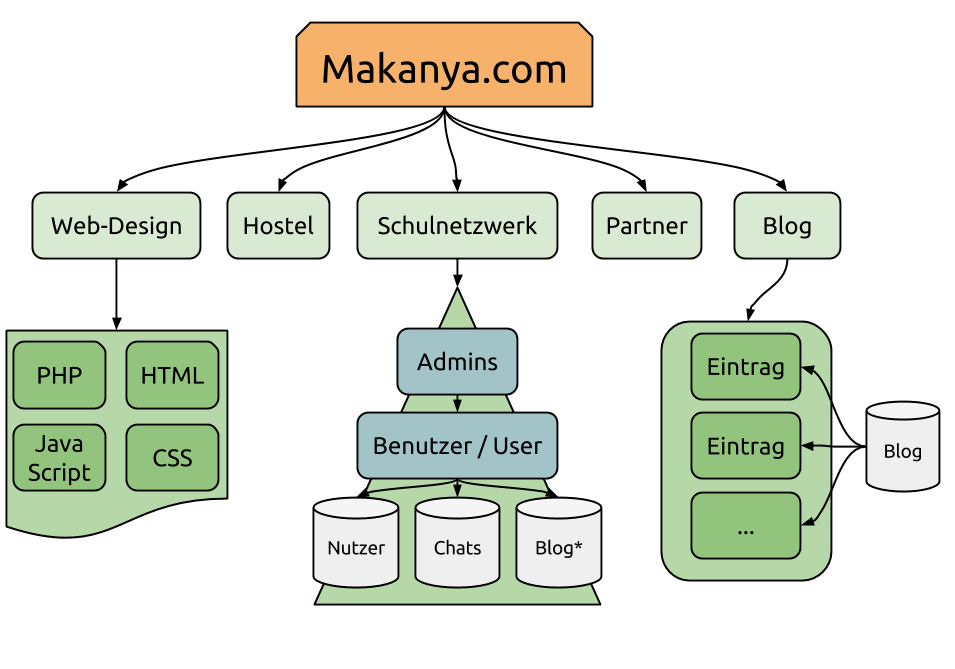
\includegraphics[width=\linewidth]{imgs/makanyaOverview.png}
\end{center}
